% !TeX program = xelatex
% !BIB program = biber
\documentclass[light]{lutbeamer}

\usepackage{pgfpages}
\usepackage{ragged2e}
\usepackage{booktabs}
\usepackage{amssymb}
\usepackage{fontawesome5}
\usepackage{tikz}
\usepackage{pgfplots}
\pgfplotsset{compat=1.18}
\addbibresource{references.bib}

% ===================================================================
% METADATA (DERS KİMLİK BİLGİLERİ)
% ===================================================================
\setdepartment{OSTİM TEKNİK ÜNİVERSİTESİ}
\institute[Yazılım Mühendisliği]{YAZILIM MÜHENDİSLİĞİ BÖLÜMÜ}
\author[Mühendislik Fakültesi]{\\
Prof.~Dr.~Yalçın ATA \\
Prof.~Dr.~Arif DEMİR \\
Dr.~Öğr.~Üyesi~Muhammed ELMNEFİ \\
Dr.~Öğr.~Üyesi~Haydar KILIÇ \\
Dr.~Öğr.~Üyesi~Emel GÜVEN \\
Dr.~Öğr.~Üyesi~Ufuk ASIL \\
Öğr.~Gör.~Sema ÇİFTÇİ
}
\title{MATH 204 -- Olasılık ve İstatistik}
\subtitle{Hafta 1: Olasılığa giriş, kümeler ve örneklem uzayı}
\date{2025--2026 Bahar Dönemi}

% ===================================================================
% OTOMATİK İÇİNDEKİLER (SUNUM AKIŞI)
% ===================================================================
\setcounter{tocdepth}{2}

\AtBeginSection[]{
  \begin{frame}{Sunum Akışı}
    \scriptsize
    \begin{columns}[T]
      \begin{column}{0.48\textwidth}
        \tableofcontents[sections={1-3}, currentsection]
      \end{column}
      \begin{column}{0.48\textwidth}
        \tableofcontents[sections={4-10}, currentsection]
      \end{column}
    \end{columns}
  \end{frame}
}

\begin{document}

\setbeamertemplate{navigation symbols}{}

% ===================================================================
% KAPAK SLAYTLARI
% ===================================================================

% Görsel Tam Kapak (Logolu)
\begin{frame}<article:0>[plain,noframenumbering]
    \begin{tikzpicture}[remember picture,overlay]
        \node[anchor=center, at=(current page.center), inner sep=0pt] {
            \includegraphics[width=\paperwidth, height=\paperheight]{logos/background_figure.jpg}
        };
    \end{tikzpicture}
\end{frame}

% Resmi Başlık Sayfası
\maketitle{}

% GENEL İÇERİK HARİTASI
\begin{frame}{İçindekiler}
  \scriptsize
  \begin{columns}[T]
    \begin{column}{0.48\textwidth}
      \tableofcontents[sections={1-3}]
    \end{column}
    \begin{column}{0.48\textwidth}
      \tableofcontents[sections={4-10}]
    \end{column}
  \end{columns}
\end{frame}

% ===================================================================
% İÇERİK: HAFTA 1
% ===================================================================

\section{Derse Giriş ve Motivasyon}
\subsection{Olasılık--İstatistik İlişkisi}
\begin{frame}{Motivasyon: Belirsizliğin Bilimi}
    \begin{columns}[T]
        \begin{column}{0.48\textwidth}
            \begin{block}{Neden Olasılık?}
                Belirsizliği modellemek, sadece yazı-tura atmak değil, modern bilimin ve mühendisliğin temelidir.
            \end{block}
            
            \begin{itemize}
                \item \textbf{Kuantum Mekaniği:} Evren deterministik değil, olasılıksaldır (Schrödinger'in kedisi).
                \item \textbf{Kriptografi:} Güvenli iletişim, şifrenin kırılma olasılığının "imkansıza yakın" olmasına dayanır.
                \item \textbf{Finans Mühendisliği:} Risk yönetimi, sigorta primleri ve borsa modelleri tamamen olasılık üzerine kuruludur.
            \end{itemize}
        \end{column}
        \begin{column}{0.48\textwidth}
            \begin{center}
                \includegraphics[width=\textwidth]{figures/week1_motivation_icon.png}
                
                \vspace{0.3cm}
                \tiny \textit{Olasılık: Kaostan düzene geçişin dili.}
            \end{center}
        \end{column}
    \end{columns}
\end{frame}

\begin{frame}{Dersin Amacı ve İzlenecek Rota}
    \begin{block}{Bu dersin ana amacı}
        Belirsizlik altında doğru model kurmak, veriyi bu modelle okumak ve
        karar verirken nicel (sayısal) gerekçe sunabilmektir.
    \end{block}

    \begin{itemize}
        \item \textbf{Hafta 1 odak}: Küme dili, olay kavramı, örneklem uzayı.
        \item \textbf{Hafta 2--3 köprü}: Olasılık kuralları, koşullu olasılık, bağımsızlık, Bayes.
        \item \textbf{Devam eden hedef}: Bu yapıyı kullanarak tahmin, karşılaştırma ve çıkarım.
    \end{itemize}

    \begin{alertblock}{Ders sonunda beklenen yetkinlik}
        Bir problemi ``deney $\rightarrow$ örneklem uzayı $\rightarrow$ olay $\rightarrow$ olasılık'' zinciriyle
        formüle edip, sonucu teknik ve anlaşılır biçimde yorumlayabilmek.
    \end{alertblock}
\end{frame}

\begin{frame}{Olasılık Neden ``Temel Dil''dir? (İstatistiksel Çıkarıma Köprü) - I}
    \begin{block}{Kavramsal köprü}
        \textbf{Olasılık} modelin dilidir (belirsizlik nasıl üretiliyor?). \\
        \textbf{İstatistik} bu dili veriye uygular (gözlenen veri modelle ne kadar uyumlu?).
    \end{block}

    \begin{exampleblock}{Örnek soru (başlangıç seviyesi)}
        Bir kalite kontrol sürecinde tek bir ürün için
        \textbf{kusurlu olayı} $K$ ile gösterilsin.
        Bu durumda \textbf{kusursuz olayı} $K'$ olur.
        Geçmiş veriye göre $P(K)=0.08$.
        \begin{itemize}
            \item Rastgele seçilen bir ürünün kusursuz olma olasılığı nedir?
            \item Bu sonuç karar verme açısından ne söyler?
        \end{itemize}
    \end{exampleblock}
\end{frame}

\begin{frame}{Olasılık Neden ``Temel Dil''dir? (İstatistiksel Çıkarıma Köprü) - II}
    \begin{block}{Çözüm ve yorum}
        \[
            P(K')=1-P(K)=1-0.08=0.92.
        \]
        Yorum: Tek bir ürünün kusursuz gelme olasılığı yüksek (\%92) olsa da,
        süreçte \%8 kusur riski vardır.
    \end{block}

    \begin{alertblock}{Karar bağlamı}
        Bu bilgi; kabul-red eşikleri, test sıklığı ve iyileştirme maliyeti
        kararları için temel girdidir.
    \end{alertblock}
\end{frame}

\subsection{Pekiştirme Soruları (Sıra Sizde)}

\begin{frame}{Soru 1: Süreç Verimliliği (Yield) ve Olasılık Yorumu}
    Bir yarı iletken fabrikasında üretilen çiplerin \%95'inin testlerden başarıyla geçtiği (yield) bilinmektedir ($P(\text{Başarılı})=0.95$).
    
    \textbf{Soru:}
    \begin{enumerate}
        \item[(a)] Rastgele seçilen bir çipin \textbf{arızalı} olma olasılığı nedir?
        \item[(b)] Bu olasılık değerine dayanarak, günlük 100.000 çip üretilen bir tesiste yaklaşık kaç adet arızalı ürün beklersiniz?
        \item[(c)] Bu sonuç bir \textbf{kesinlik} (determinism) mi, yoksa bir \textbf{beklenti} (expectation) mi ifade eder?
    \end{enumerate}
\end{frame}

\begin{frame}{Soru 1: Çözüm}
    \color{red}
    \small
    \textbf{Verilen:} $P(\text{Başarılı})=0.95$
    
    \textbf{(a) Arızalı olma olasılığı}
    \[
    P(\text{Arızalı})=1-P(\text{Başarılı})=1-0.95=0.05=\%5
    \]
    
    \textbf{(b) Günlük beklenen arızalı ürün sayısı}
    \[
    100{,}000 \times 0.05 = 5{,}000
    \]
    Yani yaklaşık \textbf{5000} adet arızalı ürün beklenir.
    
    \textbf{(c) Yorum}
    Bu değer bir \textbf{kesinlik} değil, uzun dönem ortalaması için bir \textbf{beklenti}dir.
    
    \[
    \boxed{P(\text{Arızalı})=0.05,\ \text{Beklenen sayı}\approx 5000}
    \]
\end{frame}

\section{Kümeler ve Notasyon (Set Basics)}
\subsection{Temel Kavramlar}
\begin{frame}[fragile]{Küme, Eleman, Altküme, Eşitlik, Boş Küme ($\emptyset$) Kavramı}
    \begin{columns}[T]
        \begin{column}{0.53\textwidth}
            \begin{block}{Temel tanımlar}
                \textbf{Küme}: İyi tanımlı nesneler topluluğu. \\
                \textbf{Eleman}: Kümenin bir üyesi ($x \in A$). \\
                \textbf{Altküme}: $A$'nın her elemanı $B$'de ise $A \subseteq B$. \\
                \textbf{Eşitlik}: $A=B \iff (A\subseteq B \ \text{ve}\ B\subseteq A)$. \\
                \textbf{Boş küme}: Elemanı olmayan küme, $\emptyset$.
            \end{block}

            \begin{exampleblock}{Örnek okuma}
                $2\in A$, $5\notin A$, $A\subseteq B$, $A\neq B$, $\emptyset\subseteq A$.
            \end{exampleblock}
        \end{column}
        \begin{column}{0.45\textwidth}
            \centering
            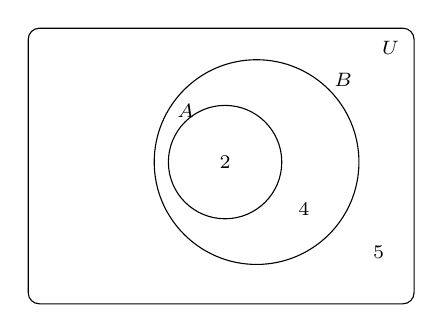
\begin{tikzpicture}[x=1cm,y=1cm,every node/.style={font=\scriptsize}]
                \draw[rounded corners] (0,0) rectangle (4.9,3.5);
                \node at (4.6,3.25) {$U$};

                \draw (2.9,1.8) circle (1.3);
                \node at (4.0,2.85) {$B$};

                \draw (2.5,1.8) circle (0.72);
                \node at (2.0,2.45) {$A$};

                \node at (2.5,1.8) {$2$};
                \node at (3.5,1.2) {$4$};
                \node at (4.45,0.65) {$5$};
            \end{tikzpicture}
        \end{column}
    \end{columns}
\end{frame}

\begin{frame}{Evrensel Küme ve Problem-Bağlamına Göre Evrensel Küme Seçimi}
    \small
    \begin{columns}[T]
        \begin{column}{0.54\textwidth}
            \begin{block}{Evrensel küme ($U$)}
                İncelenen probleme göre ``tüm olası nesneleri'' içeren referans kümedir.
                Aynı sembol farklı bağlamlarda farklı $U$ anlamına gelebilir.
            \end{block}

            \begin{itemize}
                \item Zar problemi: $U=\{1,2,3,4,5,6\}$.
                \item Sınıf problemi: $U=$ derse kayıtlı tüm öğrenciler.
                \item Üretim problemi: $U=$ incelenen partideki tüm ürünler.
            \end{itemize}

            \begin{alertblock}{Kritik nokta}
                Olayı tanımlamadan önce $U$ net seçilmezse, aynı ifade farklı sonuç verir.
            \end{alertblock}
        \end{column}
        \begin{column}{0.44\textwidth}
            \centering
            \begin{tikzpicture}[x=1cm,y=1cm,every node/.style={font=\scriptsize}]
                \draw[rounded corners, fill=blue!6] (0,1.9) rectangle (4.8,3.4);
                \node[align=left] at (2.4,2.95) {$U_1=\{1,\dots,6\}$};
                \node[align=left] at (2.4,2.35) {$A_{\text{çift}}=\{2,4,6\}$};

                \draw[rounded corners, fill=green!6] (0,0.1) rectangle (4.8,1.6);
                \node[align=left] at (2.4,1.15) {$U_2=\{1,\dots,10\}$};
                \node[align=left] at (2.4,0.55) {$A_{\text{çift}}=\{2,4,6,8,10\}$};
            \end{tikzpicture}
        \end{column}
    \end{columns}

\end{frame}

\subsection{Küme Gösterimleri}
\begin{frame}{Listeleme (Roster) ve Tanımlama (Set-Builder) Gösterimi}
    \begin{columns}[T]
        \begin{column}{0.53\textwidth}
            \begin{block}{İki temel gösterim}
                \textbf{Listeleme (roster)}: Elemanlar tek tek yazılır. \\
                \textbf{Tanımlama (set-builder)}: Özellik ile tanımlanır.
            \end{block}

            \[
                A=\{2,4,6,8\}
                \]
                \[
                B=\{x \in \mathbb{N} \mid 1\le x<10,\ x \text{ çift}\}
            \]

            \begin{exampleblock}{Yorum}
                $A$ ve $B$ aynı kümeyi farklı gösterimlerle verir.
            \end{exampleblock}
        \end{column}
        \begin{column}{0.45\textwidth}
            \centering
            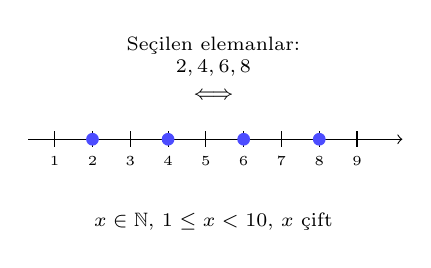
\begin{tikzpicture}[x=0.48cm,y=1cm,every node/.style={font=\scriptsize}]
                \draw[->] (0.3,0) -- (10.2,0);
                \foreach \x in {1,...,9}{
                    \draw (\x,0.1) -- (\x,-0.1);
                    \node[below] at (\x,-0.1) {\tiny \x};
                }
                \foreach \x in {2,4,6,8}{
                    \fill[blue!70] (\x,0) circle (2.3pt);
                }
                \node[align=center] at (5.2,1.05) {Seçilen elemanlar:\\$2,4,6,8$};
                \node at (5.2,0.55) {$\Longleftrightarrow$};
                \node[align=center] at (5.2,-1.05) {$x\in\mathbb{N}$, $1\le x<10$, $x$ çift};
            \end{tikzpicture}
        \end{column}
    \end{columns}
\end{frame}

\begin{frame}{Sık Yapılan Hatalar: ``Tanımlama Kümesi'' vs ``Özellik''}
    \begin{columns}[T]
        \begin{column}{0.53\textwidth}
            \begin{block}{Yaygın hata}
                $\{x \mid \text{özellik}\}$ yazarken, $x$'in hangi kümeden geldiği
                belirtilmezse ifade belirsiz olabilir.
            \end{block}

            \begin{itemize}
                \item Hatalı/eksik: $\{x \mid x^2=1\}$.
                \item Doğru 1: $\{x\in\mathbb{R}\mid x^2=1\}=\{-1,1\}$.
                \item Doğru 2: $\{x\in\mathbb{N}\mid x^2=1\}=\{1\}$.
            \end{itemize}

            \begin{alertblock}{Pratik kural}
                Önce ``tanımlama kümesi'', sonra ``özellik'' yaz.
            \end{alertblock}
        \end{column}
        \begin{column}{0.45\textwidth}
            \centering
            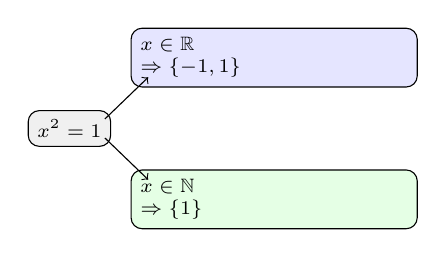
\begin{tikzpicture}[x=1cm,y=1cm,every node/.style={font=\scriptsize}]
                \node[draw, rounded corners, fill=gray!12] (exp) at (0,0) {$x^2=1$};
                \node[draw, rounded corners, fill=blue!10, align=left, text width=3.4cm] (r) at (2.6,0.9)
                {$x\in\mathbb{R}$\\$\Rightarrow \{-1,1\}$};
                \node[draw, rounded corners, fill=green!10, align=left, text width=3.4cm] (n) at (2.6,-0.9)
                {$x\in\mathbb{N}$\\$\Rightarrow \{1\}$};
                \draw[->] (0.45,0.12) -- (1.0,0.65);
                \draw[->] (0.45,-0.12) -- (1.0,-0.65);
            \end{tikzpicture}
        \end{column}
    \end{columns}
\end{frame}

\subsection{Küme İşlemleri}
\begin{frame}[fragile]{Birleşim ($\cup$), Kesişim ($\cap$), Fark, Tümleyen (Complement)}
    \scriptsize
    \begin{columns}[T]
        \begin{column}{0.54\textwidth}
            \begin{block}{İşlem anlamları}
                \[
                    \begin{aligned}
                        A\cup B &: \text{A veya B (ya da ikisi)}\\
                        A\cap B &: \text{A ve B}\\
                        A\setminus B &: \text{A'da olup B'de olmayanlar}\\
                        A' &: \text{U içinde A'nın tümleyeni}
                    \end{aligned}
                \]
            \end{block}

            \begin{exampleblock}{Örnek}
                $U=\{1,2,3,4,5,6\}$, $A=\{1,2,3,4\}$, $B=\{3,4,5\}$:
                \[
                    \begin{aligned}
                        A\cup B&=\{1,2,3,4,5\},\quad A\cap B=\{3,4\},\\
                        A\setminus B&=\{1,2\},\quad A'=\{5,6\}
                    \end{aligned}
                \]
            \end{exampleblock}
        \end{column}
        \begin{column}{0.44\textwidth}
            \centering
            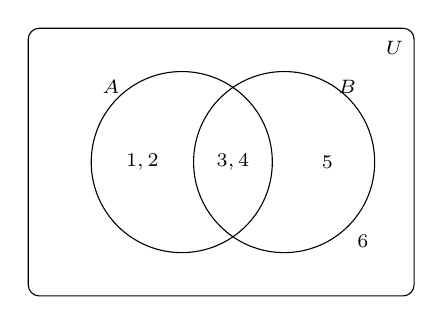
\begin{tikzpicture}[x=1cm,y=1cm,every node/.style={font=\scriptsize}]
                \draw[rounded corners] (0,0) rectangle (4.9,3.4);
                \node at (4.65,3.15) {$U$};

                \draw (1.95,1.7) circle (1.15);
                \draw (3.25,1.7) circle (1.15);
                \node at (1.05,2.65) {$A$};
                \node at (4.05,2.65) {$B$};

                \node at (1.45,1.7) {$1,2$};
                \node at (2.6,1.7) {$3,4$};
                \node at (3.8,1.7) {$5$};
                \node at (4.25,0.7) {$6$};
            \end{tikzpicture}
        \end{column}
    \end{columns}
\end{frame}

\begin{frame}{Tümleyen Kavramı ve Örnekler}
    \begin{block}{Tümleyen sezgisi}
        Bir olayın olmaması, tümleyen olaydır.
        Olasılıkta temel bağıntı: $P(A')=1-P(A)$.
    \end{block}

    \begin{exampleblock}{Örnek soru}
        Bir üretim hattında ürünün kusurlu olma olasılığı $P(K)=0.07$.
        Kusursuz olma olasılığı nedir?
    \end{exampleblock}

    \begin{block}{Çözüm}
        \[
            P(K')=1-P(K)=1-0.07=0.93.
        \]
    \end{block}
\end{frame}

\begin{frame}{Kesişim Kavramı ve Örnekler}
    \begin{block}{Kesişim}
        $A\cap B$, iki koşulun aynı anda sağlandığı sonuç kümesidir.
    \end{block}

    \begin{exampleblock}{Örnek}
        $U=\{1,2,3,4,5,6\}$ olsun. \\
        $A=$ ``çift gelme'' $=\{2,4,6\}$, 
        $B=$ ``3'ten büyük gelme'' $=\{4,5,6\}$.
        \[
            A\cap B=\{4,6\}.
        \]
        Yani hem çift hem 3'ten büyük sonuçlar.
    \end{exampleblock}
\end{frame}

\subsection{Ayrık (Disjoint) Kümeler ve Parçalama (Partition)}
\begin{frame}{Ayrık/Çakışmayan (Mutually Exclusive) Olay Fikri}
    \begin{block}{Tanım}
        $A$ ve $B$ ayrık ise $A\cap B=\emptyset$.
        Aynı anda gerçekleşmeleri mümkün değildir.
    \end{block}

    \begin{itemize}
        \item Zar atışında $A=$ ``tek'', $B=$ ``çift'' $\Rightarrow$ ayrık.
        \item $A=$ ``çift'', $C=$ ``3'ten büyük'' $\Rightarrow$ ayrık değil.
    \end{itemize}

    \begin{alertblock}{Sık karışan nokta}
        Ayrıklık, bağımsızlık değildir.
        Eğer $P(A)>0$ ve $P(B)>0$ iken $A\cap B=\emptyset$ ise
        $P(A\cap B)=0$ olur; fakat $P(A)P(B)>0$ olduğundan bağımsızlık sağlanmaz.
    \end{alertblock}
\end{frame}

\begin{frame}{Partition (Örneklem Uzayını Ayrık Parçalara Bölme) Fikri}
    \begin{columns}[T]
        \begin{column}{0.46\textwidth}
            \begin{block}{Partition (parçalama)}
                $\{B_1,B_2,\dots,B_k\}$ bir partition ise:
                \begin{itemize}
                    \item Her $B_i\neq \emptyset$,
                    \item $B_i$'ler ikili olarak ayrık,
                    \item $\bigcup_{i=1}^k B_i=U$.
                \end{itemize}
                Yani örneklem uzayı örtüşmeyen parçalara ayrılır.
            \end{block}
        \end{column}
        \begin{column}{0.52\textwidth}
            \centering
            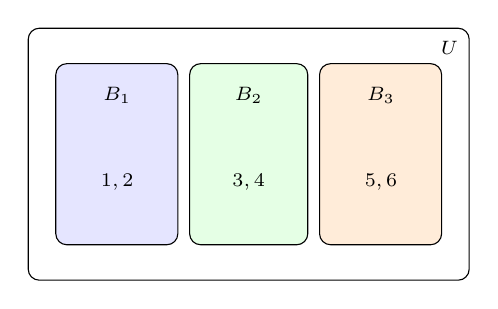
\begin{tikzpicture}[x=1cm,y=1cm,every node/.style={font=\scriptsize}]
                \draw[rounded corners] (0,0) rectangle (5.6,3.2);
                \node at (5.35,2.95) {$U$};

                \draw[rounded corners, fill=blue!10] (0.35,0.45) rectangle (1.9,2.75);
                \draw[rounded corners, fill=green!10] (2.05,0.45) rectangle (3.55,2.75);
                \draw[rounded corners, fill=orange!15] (3.7,0.45) rectangle (5.25,2.75);

                \node at (1.13,2.35) {$B_1$};
                \node at (2.8,2.35) {$B_2$};
                \node at (4.48,2.35) {$B_3$};

                \node at (1.13,1.25) {$1,2$};
                \node at (2.8,1.25) {$3,4$};
                \node at (4.48,1.25) {$5,6$};
            \end{tikzpicture}

            \vspace{0.12cm}
            {\tiny Örnek: $U=\{1,2,3,4,5,6\}$ için $B_1,B_2,B_3$ örtüşmeden $U$'yu kaplar.}
        \end{column}
    \end{columns}

    \vspace{0.3cm}
    \begin{block}{Neden önemli?}
        Toplam olasılık ve Bayes teoremi gibi konuların temel yapısını oluşturur.
    \end{block}
\end{frame}

\subsection{Pekiştirme Soruları (Sıra Sizde)}

\begin{frame}{Soru 2: Küme İşlemleri ve Parçalama}
    $U=\{x \in \mathbb{Z} \mid 1 \le x \le 10\}$ evrensel kümesi verilsin.
    \[
        A=\{x \in U \mid x \text{ asal sayı}\}, \quad
        B=\{x \in U \mid x \text{ çift sayı}\}
    \]
    kümeleri tanımlanıyor.
    
    \textbf{Soru:}
    \begin{enumerate}
        \item[(a)] $A$ ve $B$ kümelerini liste yöntemiyle yazınız.
        \item[(b)] $A \cap B$ kümesi nedir? Bu iki küme \textbf{ayrık} mıdır?
        \item[(c)] $C=\{1,9\}$ kümesi tanımlansın. $\{A,B,C\}$ koleksiyonu $U$ için bir \textbf{parçalanış} (partition) oluşturur mu? Neden?
    \end{enumerate}
\end{frame}

\begin{frame}{Soru 2: Çözüm}
    \color{red}
    \small
    \[
    U=\{1,2,3,4,5,6,7,8,9,10\}
    \]
    
    \textbf{(a) Liste yöntemi}
    \[
    A=\{2,3,5,7\}\ (\text{asallar}),\qquad
    B=\{2,4,6,8,10\}\ (\text{çiftler})
    \]
    
    \textbf{(b) Kesişim ve ayrıklık}
    \[
    A\cap B=\{2\}
    \]
    Kesişim boş olmadığı için $A$ ve $B$ \textbf{ayrık değildir}.
    
    \textbf{(c) Partition kontrolü}, $C=\{1,9\}$
    \[
    A\cap B=\{2\}\neq \emptyset
    \]
    Bu tek başına partition olmayı bozar (ikili ayrıklık şartı sağlanmıyor).
    Ayrıca $A\cup B\cup C=U$ olsa bile ayrıklık sağlanmadığı için partition değildir.
    
    \[
    \boxed{\{A,B,C\}\ \text{partition değildir}}
    \]
\end{frame}

\section{Olasılık Deneyi ve Örneklem Uzayı (Sample Space)}
\subsection{Deney--Çıktı--Örneklem Uzayı}
\begin{frame}{İstatistiksel Deney (Experiment) ve Çıktı (Outcome) Dili}
    \begin{block}{Deney dili}
        \textbf{İstatistiksel deney}, sonucu kesin öngörülemeyen ama olası sonuçları
        tanımlanabilen süreçtir.
        Her tekil sonuç bir \textbf{çıktı}dır (outcome).
    \end{block}

    \begin{itemize}
        \item Para atışı: çıktılar $T$ (Tura) veya $Y$ (Yazı).
        \item Üretim kontrolü: çıktı ``kusurlu'' veya ``kusursuz''.
        \item Ölçüm deneyi: çıktı sayısal değer (örn. sıcaklık, süre).
    \end{itemize}

    \begin{alertblock}{Amaç}
        Deneyi doğru tanımlamak, sonraki olasılık modelinin temelini oluşturur.
    \end{alertblock}
\end{frame}

\begin{frame}{Örneklem Uzayı Tanımı ve Örnek Nokta (Sample Point)}
    \begin{block}{Tanım}
        Bir deneyin tüm olası çıktılar kümesine \textbf{örneklem uzayı} denir ve
        genellikle $S$ ile gösterilir.
        $S$ içindeki her elemana \textbf{örnek nokta} denir.
    \end{block}

    \begin{exampleblock}{Örnek}
        Zar atışı için:
        \[
            S=\{1,2,3,4,5,6\}
        \]
        Burada her sayı bir örnek noktadır.
    \end{exampleblock}
\end{frame}

\begin{frame}[fragile]{Aynı Deney İçin Farklı Örneklem Uzayı Seçimi ($S_1$ vs $S_2$)}
    \begin{block}{Aynı deney, farklı temsil}
        Aynı fiziksel süreç farklı ayrıntı düzeylerinde modellenebilir.
        Zar deneyi için:
        \[
            S_1=\{1,2,3,4,5,6\}, \qquad
            S_2=\{\text{tek},\text{çift}\}
        \]
        $S_2$, $S_1$ üzerindeki ``tek/çift'' sınıflandırmasının daha kaba halidir.
    \end{block}

    \begin{itemize}
        \item Sonucun \textbf{tam değerini} soruyorsanız $S_1$ gerekir.
        \item Sadece \textbf{tek-çift} bilgisi gerekiyorsa $S_2$ yeterlidir.
        \item Problem hangi ayrıntıyı gerektiriyorsa o uzay seçilir.
    \end{itemize}
\end{frame}

\begin{frame}{``Bilgi Granülerliği'' ve Örneklem Uzayını Doğru Seçme}
    \begin{block}{Granülerlik ilkesi}
        Çok kaba örneklem uzayı önemli ilişkileri gizleyebilir; çok detaylı uzay ise
        hesaplamayı gereksiz zorlaştırabilir.
    \end{block}

    \begin{exampleblock}{Uygulama kuralı}
        Soruda hangi olasılık isteniyorsa, o olayı doğal biçimde ifade edecek en küçük
        ama yeterli örneklem uzayı seçilir.
    \end{exampleblock}
\end{frame}

\subsection{Örneklem Uzayı Kurma Teknikleri}
\begin{frame}{Sistematik Listeleme Stratejileri}
    \begin{block}{Sistematik üretim}
        Sonuçları rastgele yazmak yerine düzenli bir kural izlenir:
        sıralama, tablo, kodlama veya bloklama.
    \end{block}

    \begin{exampleblock}{Örnek}
        İki para atışında olası sonuçlar:
        \[
            S=\{TT,TY,YT,YY\}
        \]
        İlk harf 1. atışı, ikinci harf 2. atışı temsil eder.
    \end{exampleblock}
\end{frame}

\begin{frame}{Ağaç Diyagramı ile Örneklem Uzayı Üretme}
    \begin{columns}[T]
        \begin{column}{0.45\textwidth}
            \begin{block}{Yöntem}
                Ağaç diyagramında:
                \begin{itemize}
                    \item Her seviye bir adımı,
                    \item Her dal olası sonucu,
                    \item Her tam yol bir örnek noktayı verir.
                \end{itemize}
            \end{block}

            \begin{exampleblock}{Örnek (koşullu deney)}
                Önce para atılıyor. İlk atış $T$ ise tekrar para, $Y$ ise zar atılıyor.
                \[
                    S=\{TT,TY,Y1,Y2,Y3,Y4,Y5,Y6\}
                \]
            \end{exampleblock}
        \end{column}
        \begin{column}{0.53\textwidth}
            \centering
            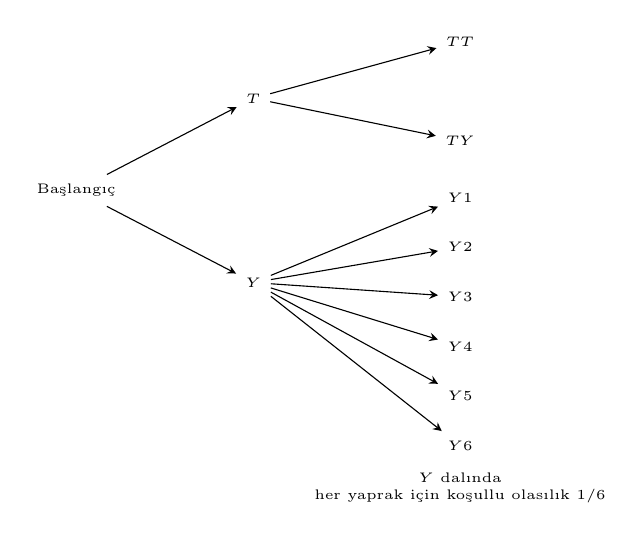
\begin{tikzpicture}[x=1.25cm,y=0.9cm,>=stealth, every node/.style={font=\tiny}]
                \node (r) at (0,0) {Başlangıç};
                \node (t) at (1.8,1.3) {$T$};
                \node (y) at (1.8,-1.3) {$Y$};

                \draw[->] (r) -- (t);
                \draw[->] (r) -- (y);

                \node (tt) at (3.9,2.1) {$TT$};
                \node (ty) at (3.9,0.7) {$TY$};
                \draw[->] (t) -- (tt);
                \draw[->] (t) -- (ty);

                \node (y1) at (3.9,-0.1) {$Y1$};
                \node (y2) at (3.9,-0.8) {$Y2$};
                \node (y3) at (3.9,-1.5) {$Y3$};
                \node (y4) at (3.9,-2.2) {$Y4$};
                \node (y5) at (3.9,-2.9) {$Y5$};
                \node (y6) at (3.9,-3.6) {$Y6$};

                \draw[->] (y) -- (y1);
                \draw[->] (y) -- (y2);
                \draw[->] (y) -- (y3);
                \draw[->] (y) -- (y4);
                \draw[->] (y) -- (y5);
                \draw[->] (y) -- (y6);

                \node[align=center] at (3.9,-4.2) {$Y$ dalında\\her yaprak için koşullu olasılık $1/6$};
            \end{tikzpicture}
        \end{column}
    \end{columns}
\end{frame}

\begin{frame}{Ağaç Diyagramı: Yol--Örnek Nokta Eşlemesi}
    \begin{columns}[T]
        \begin{column}{0.46\textwidth}
            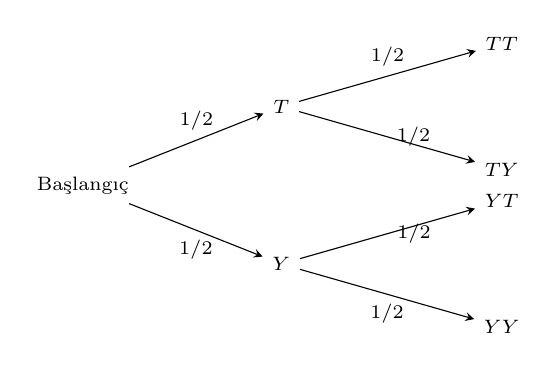
\begin{tikzpicture}[x=1.4cm,y=1.0cm,>=stealth, every node/.style={font=\scriptsize}]
                \node (r) at (0,0) {Başlangıç};
                \node (t1) at (1.8,1.0) {$T$};
                \node (y1) at (1.8,-1.0) {$Y$};
                \draw[->] (r) -- (t1) node[midway,above] {$1/2$};
                \draw[->] (r) -- (y1) node[midway,below] {$1/2$};

                \node (tt) at (3.8,1.8) {$TT$};
                \node (ty) at (3.8,0.2) {$TY$};
                \node (yt) at (3.8,-0.2) {$YT$};
                \node (yy) at (3.8,-1.8) {$YY$};

                \draw[->] (t1) -- (tt) node[midway,above] {$1/2$};
                \draw[->] (t1) -- (ty) node[midway,right] {$1/2$};
                \draw[->] (y1) -- (yt) node[midway,right] {$1/2$};
                \draw[->] (y1) -- (yy) node[midway,below] {$1/2$};
            \end{tikzpicture}
        \end{column}
        \begin{column}{0.52\textwidth}
            \begin{block}{Okuma prensibi (iki para örneği)}
                Ağaçta her tam yol bir birleşik çıktıdır.
                Yol sırası, deney adımlarının sırasıdır.
            \end{block}

            \begin{itemize}
                \item Kök $\rightarrow T \rightarrow Y$ yolu: $TY$
                \item Kök $\rightarrow Y \rightarrow T$ yolu: $YT$
                \item Tüm yapraklar birleştirilince: $S=\{TT,TY,YT,YY\}$
            \end{itemize}

            \begin{alertblock}{Kontrol}
                Tüm yapraklar listelendi mi? Aynı yaprak iki kez yazıldı mı?
            \end{alertblock}
        \end{column}
    \end{columns}
\end{frame}

\subsection{Pekiştirme Soruları (Sıra Sizde)}

\begin{frame}{Soru 3: Ağaç Diyagramı ile Örneklem Uzayı}
    Bir torbada 3 kırmızı (K) ve 2 mavi (M) top vardır. Torbadan \textbf{iade edilmeksizin} (without replacement) art arda iki top çekiliyor.
    Bu soruda \textbf{top kimliği değil, sadece renk sırası} kaydedilmektedir.
    
    \textbf{Soru:}
    \begin{enumerate}
        \item[(a)] Bu deneyin tüm olası çıktılarını (örneklem uzayını) bir ağaç diyagramı çizerek belirleyiniz.
        \item[(b)] $S$ kümesini liste yöntemiyle yazınız.
        \item[(c)] ``En az bir mavi top gelmesi'' olayını ($E$) küme olarak ifade ediniz.
    \end{enumerate}
\end{frame}

\begin{frame}{Soru 3: Çözüm}
    \color{red}
    \small
    \textbf{Deney:} 3 kırmızı (K), 2 mavi (M) toptan iadesiz 2 çekim.

    \begin{columns}[T]
        \begin{column}{0.50\textwidth}
            \centering
            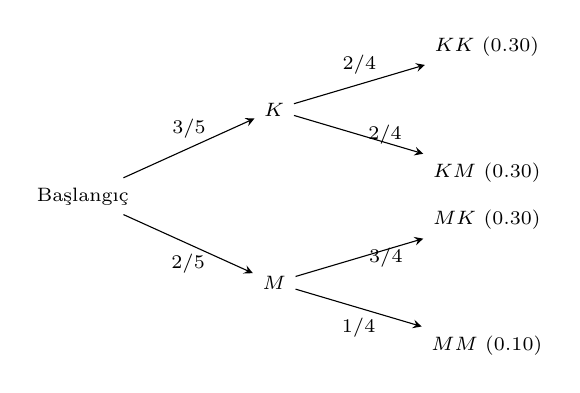
\begin{tikzpicture}[x=1.35cm,y=1.0cm,>=stealth, every node/.style={font=\scriptsize}]
                \node (r) at (0,0) {Başlangıç};
                \node (k1) at (1.8,1.1) {$K$};
                \node (m1) at (1.8,-1.1) {$M$};

                \draw[->] (r) -- (k1) node[midway,above] {$3/5$};
                \draw[->] (r) -- (m1) node[midway,below] {$2/5$};

                \node (kk) at (3.8,1.9) {$KK\ (0.30)$};
                \node (km) at (3.8,0.3) {$KM\ (0.30)$};
                \node (mk) at (3.8,-0.3) {$MK\ (0.30)$};
                \node (mm) at (3.8,-1.9) {$MM\ (0.10)$};

                \draw[->] (k1) -- (kk) node[midway,above] {$2/4$};
                \draw[->] (k1) -- (km) node[midway,right] {$2/4$};
                \draw[->] (m1) -- (mk) node[midway,right] {$3/4$};
                \draw[->] (m1) -- (mm) node[midway,below] {$1/4$};
            \end{tikzpicture}
        \end{column}
        \begin{column}{0.48\textwidth}
            \textbf{(a) Ağaçtan gelen renk sıraları}
            \[
            KK,\ KM,\ MK,\ MM
            \]

            \textbf{(b) Örneklem uzayı}
            \[
            S=\{KK,KM,MK,MM\}
            \]
            Not: Örnek noktalar \textbf{eş olasılıklı değildir}.

            \textbf{(c) En az bir mavi}
            \[
            E=\{KM,MK,MM\}
            \]
        \end{column}
    \end{columns}

    \[
    \boxed{S=\{KK,KM,MK,MM\},\quad E=\{KM,MK,MM\}}
    \]
\end{frame}

\section{Olay (Event) Kavramı ve Olay Cebiri}
\subsection{Olay = Alt-Küme}
\begin{frame}{Olayın Örneklem Uzayının Alt-Kümesi Olarak Okunması}
    \begin{block}{Tanım}
        \textbf{Olay}, örneklem uzayının bir altkümesidir.
        Yani olay gerçekleşirse, gözlenen sonuç o altkümenin bir elemanıdır.
    \end{block}

    \begin{exampleblock}{Örnek}
        Zar için $S=\{1,2,3,4,5,6\}$.
        ``3'e bölünebilme'' olayı:
        \[
            A=\{3,6\}\subseteq S.
        \]
    \end{exampleblock}
\end{frame}

\begin{frame}[fragile]{Boş Olay ($\emptyset$) ve Kesin Olay ($S$) Sezgisi}
    \begin{block}{İki uç durum}
        \textbf{Boş olay} $\emptyset$: hiç gerçekleşmeyen olay. \\
        \textbf{Kesin olay} $S$: daima gerçekleşen olay.
    \end{block}

    \[
        P(\emptyset)=0, \qquad P(S)=1
    \]

    \begin{exampleblock}{Örnek}
        Zar atışında ``7 gelmesi'' olayı $\emptyset$, 
        ``1 ile 6 arasında bir sayı gelmesi'' olayı $S$'dir.
    \end{exampleblock}
\end{frame}

\subsection{Olaylar Üzerinde İşlemler}
\begin{frame}{Olayların Kesişimi: ``İkisi Birden''}
    \begin{block}{Kesişim yorumu}
        $A\cap B$, hem $A$ hem $B$ olaylarının birlikte gerçekleşmesidir.
    \end{block}

    \begin{exampleblock}{Örnek}
        Zar atışında:
        \[
            A=\{2,4,6\},\quad B=\{4,5,6\}
        \]
        \[
            A\cap B=\{4,6\}.
        \]
    \end{exampleblock}
\end{frame}

\begin{frame}{Ayrık Olaylar: ``Aynı Anda Olamaz''}
    \begin{block}{Tanım}
        $A$ ve $B$ ayrık ise:
        \[
            A\cap B=\emptyset.
        \]
        Bu olaylar aynı denemede birlikte gerçekleşemez.
    \end{block}

    \begin{exampleblock}{Örnek}
        Tek zar atışında ``tek'' ve ``çift'' olayları ayrık olaylardır.
    \end{exampleblock}
\end{frame}

\begin{frame}{Birleşim: ``En Az Biri'' (Sezgisel Okuma)}
    \begin{block}{Birleşim yorumu}
        $A\cup B$, ``$A$ veya $B$ veya her ikisi'' anlamına gelir.
    \end{block}

    \begin{exampleblock}{Örnek}
        \[
            A=\{2,4,6\},\quad B=\{4,5,6\}
        \]
        \[
            A\cup B=\{2,4,5,6\}.
        \]
    \end{exampleblock}
\end{frame}

\begin{frame}{Venn Diyagramı ile Olay İşlemleri (Görsel Temsil)}
    \begin{block}{Görselleştirme}
        Venn diyagramında dikdörtgen $S$'yi, daireler olayları temsil eder.
        Kesişim ortak bölge, birleşim kaplanan toplam bölge, tümleyen dış bölgedir.
    \end{block}

    \begin{itemize}
        \item $A\cap B$: iki dairenin ortak alanı
        \item $A\cup B$: en az bir daire içinde kalan alan
        \item $A'$: $S$ içinde $A$ dışında kalan alan
    \end{itemize}

    \begin{alertblock}{Neden kullanılır?}
        Soyut küme işlemlerini hızlı ve hatasız yorumlamak için.
    \end{alertblock}
\end{frame}

\subsection{Pekiştirme Soruları (Sıra Sizde)}

\begin{frame}{Soru 4: Olay Cebiri ve Venn Diyagramı Yorumlama}
    Bir sınıftaki öğrencilerle ilgili üç olay tanımlanmıştır:
    \begin{itemize}
        \item $M$: Matematik dersini geçenler,
        \item $F$: Fizik dersini geçenler,
        \item $K$: Kimya dersini geçenler.
    \end{itemize}
    
    \textbf{Soru:} Aşağıdaki sözel ifadeleri küme notasyonu (birleşim, kesişim, tümleyen) ile yazınız:
    \begin{enumerate}
        \item[(a)] Sadece Matematik dersini geçenler (Fizik ve Kimya'dan kalanlar).
        \item[(b)] Matematik veya Fizik dersini geçen, fakat Kimya'dan kalanlar.
        \item[(c)] Üç dersten de kalanlar.
        \item[(d)] En az iki dersten geçenler.
    \end{enumerate}
\end{frame}

\begin{frame}{Soru 4: Çözüm}
    \color{red}
    \small
    \textbf{(a) Sadece Matematik geçenler}
    \[
    M\cap F'\cap K'
    \]
    
    \textbf{(b) Matematik veya Fizik geçen, Kimya'dan kalanlar}
    \[
    (M\cup F)\cap K'
    \]
    
    \textbf{(c) Üç dersten de kalanlar}
    \[
    M'\cap F'\cap K'
    \]
    
    \textbf{(d) En az iki dersten geçenler}
    \[
    (M\cap F)\cup(M\cap K)\cup(F\cap K)
    \]
    Not: Üç dersi birden geçen öğrenciler bu kümenin içindedir; küme birleşiminde tekrar sayım problemi yoktur.
    (Eşdeğer açılım: $(M\cap F\cap K')\cup(M\cap K\cap F')\cup(F\cap K\cap M')\cup(M\cap F\cap K)$.)
    
    \[
    \boxed{\text{Tüm ifadeler küme cebiriyle yukarıdaki gibidir}}
    \]
\end{frame}

\section{Hafta 1 Kapanış}
\subsection{Özet ve Kontrol}
\begin{frame}[fragile]{Kavram Haritası: $S$, Sample Point, Event, $\cap$/$\cup$/Complement}
    \begin{block}{Hafta 1 akış özeti}
        \[
            \text{Deney} \rightarrow S \rightarrow \text{Örnek Nokta} \rightarrow \text{Olay} \rightarrow
            (\cap,\cup,')
        \]
        Bu zincir, olasılık hesabına başlamadan önceki zorunlu temel yapıdır.
    \end{block}

    \begin{itemize}
        \item Olaylar birer altkümedir.
        \item Ayrıklık, kesişimin boş olmasıdır.
        \item Partition fikri, ileri konularda (toplam olasılık/Bayes) anahtardır.
    \end{itemize}
\end{frame}

\begin{frame}{Mini-Quiz: Örneklem Uzayı/Olay Belirleme}
    \begin{exampleblock}{Soru 1}
        İki madeni para atılıyor. Örneklem uzayını yazınız.
    \end{exampleblock}

    \begin{exampleblock}{Soru 2}
        Yukarıdaki deneyde ``en az bir yazı'' olayını küme olarak yazınız.
    \end{exampleblock}

    \begin{block}{Kısa cevap}
        \[
            S=\{TT,TY,YT,YY\},\qquad
            A=\{TY,YT,YY\}.
        \]
    \end{block}
\end{frame}

\begin{frame}{Çıkış Bileti: ``Bu Hafta En Kritik 3 Cümle''}
    \begin{enumerate}
        \item Olay, örneklem uzayının bir altkümesidir.
        \item Küme işlemleri (kesişim, birleşim, tümleyen) olay cebirinin temelidir.
        \item Doğru örneklem uzayı seçimi, doğru olasılık modelinin ön koşuludur.
    \end{enumerate}

    \begin{alertblock}{Ödev yönlendirmesi}
        Her öğrenci kendi bölümünden bir deney seçip $S$, iki olay ve bir partition
        tanımlayarak bir sayfalık çözüm hazırlasın.
    \end{alertblock}
\end{frame}

\section{Kaynaklar}
\begin{frame}[allowframebreaks]{Kaynaklar}
    \nocite{*}
    \printbibliography{}
\end{frame}

\section{Haftalık Uygulama}
\begin{frame}{Sıra Sizde: Kaggle Uygulaması}
    \justifying{}
    Teoriyi pratiğe dökmek için hazırladığımız Python Notebook sizi bekliyor.
    
    \vspace{0.5cm}
    \begin{enumerate}
        \item \textbf{Adım 1:} \href{https://www.kaggle.com}{Kaggle.com} hesabınıza giriş yapın.
        \item \textbf{Adım 2:} Aşağıdaki linkten dersin defterine gidin:
        
        \vspace{0.3cm}
        \begin{center}
             \hrefcol{https://www.kaggle.com/code/ufukasil/1-hafta-olasilik-notebook}{Kaggle Notebook: Kümeler ve Olasılığa Giriş}
        \end{center}
        \vspace{0.3cm}
        
        \item \textbf{Adım 3:} Sağ üstten \textbf{"Copy \& Edit"} butonuna basarak kopyanızı oluşturun ve kodları çalıştırın.
    \end{enumerate}
\end{frame}

\section{Yapay Zeka Asistanı}
\begin{frame}{Yapay Zeka Asistanınız: NotebookLM}
    \begin{columns}[T]
        \begin{column}{0.48\textwidth}
            \justifying{}
            \textbf{Ders Materyalleri ile Etkileşime Geçin!}
            
            Bu dersin tüm içeriği (sunumlar, makaleler ve notlar), Google'ın gelişmiş yapay zeka asistanı \textbf{NotebookLM} sistemine yüklenmiştir.
            
            \vspace{1em}
            \begin{itemize}
                \item \textbf{Anında Cevaplar:} Aklınıza takılanları sorun.
                \item \textbf{Özetler:} Karmaşık konuları basitçe öğrenin.
                \item \textbf{Audio Overview:} Dersi bir podcast gibi dinleyin.
            \end{itemize}
            
            \vspace{1.5em}
            \begin{center}
                {\setbeamercolor{button}{bg=red,fg=black}
                \href{https://notebooklm.google.com/notebook/4fba83ea-866c-43ee-b8d7-9c89ae3bb471}{\beamerbutton{\rule[-4ex]{0pt}{11ex}\Large \textbf{Hemen Deneyin}}}}
            \end{center}
        \end{column}
        
        \begin{column}{0.48\textwidth}
            \centering
            \includegraphics[width=\textwidth, height=0.6\textheight, keepaspectratio]{figures/notebooklm.jpg}
        \end{column}
    \end{columns}
\end{frame}

\begin{frame}[plain,noframenumbering]
    \begin{tikzpicture}[remember picture,overlay]
        \node[anchor=center, at=(current page.center), inner sep=0pt] {
            \includegraphics[width=\paperwidth, height=\paperheight]{figures/combined_qrs.png}
        };
        \node[anchor=south, at=(current page.south), yshift=0.5cm, fill=white!95, rounded corners, inner sep=10pt, text width=0.95\paperwidth, align=center] {
            \Large \textbf{\textcolor{blue}{Bizi Takip Edin!}} \\
            \vspace{0.3em}
            \small Ders tekrarlarıyla konuları pekiştirmek (YouTube), profesyonel proje ağlarına katılmak (LinkedIn) ve kampüs duyurularından anında haberdar olmak (Instagram) için topluluğumuza katılın.
        };
    \end{tikzpicture}
\end{frame}

\end{document}
